%\documentclass[prb,11pt,notitlepage]{revtex4-1}
%\documentclass[11pt,notitlepage]{revtex4-1}
\documentclass[11pt,a4paper]{article}
%---------------------------
% preambulo:
%---------------------------
\usepackage{abstract}
\usepackage[affil-it]{authblk}
\usepackage[utf8]{inputenc}	% encoding do arquivo, reconhecimento de acentos, etc.
\usepackage[brazilian]{babel}    % hiphenação em portugues
\usepackage{textcomp} % pacote para simbolos gregos no texto, sem ficar itálico
\usepackage{amsmath}    % need for subequations
\usepackage{amssymb}    % need for math symbols
\usepackage{graphicx}   % need for figures
\usepackage{verbatim}   % useful for program listings
\usepackage{color}      % use if color is used in text
\usepackage{subfigure}  % use for side-by-side figures
\usepackage{hyperref}   % use for hypertext links, including those to external documents and URLs
\usepackage[yyyymmdd,hhmmss]{datetime} % pacote para escrever a data de hoje
\usepackage[brazilian,nameinlink]{cleveref} % pacote para referenciar figuras e equacoes
\usepackage[table,xcdraw]{xcolor} % tabelas coloridas
\usepackage{circuitikz} %Pacote para desenhar circuitos
\ctikzset{bipoles/length=0.9 cm} % tamanho dos componentes desenhados nos circuitos pelo pacote Circuitikz
\raggedbottom           % don't add extra vertical space
%---------------------------
%MARGENS
%---------------------------
\usepackage{indentfirst}        % indenta primeiro parágrafo
\setlength{\topmargin}{-15pt} % extra vert. space + at the top of header: 23pt
\setlength{\oddsidemargin}{-15pt} % extra spc added at the left of odd page: 0pt
\setlength{\textheight}{625pt} % comprimento do corpo do texto
\setlength{\textwidth}{480pt} % largura do corpo do texto
\setlength{\footskip}{50pt} % distancia da ultima linha de texto até número da pg.
%--------------------------
% INICIO DO DOCUMENTO:
%--------------------------
\begin{document}
%---------	
%cabeçalho
%---------
\title{Relatório 1: Filtros \\
\small{
F429 - G.5  2$^{ \underbar{\text{o}} }$ semestre 2015\\
Prof. Lázaro Padilha }
}
\author{Pedro Bacchi Finkler}
\affil{Universidade Estadual de Campinas, Faculdade de Engenharia Elétrica e Computação, Campinas, SP}

\date{\today}

\maketitle % forma a página de título
%---------
%Resumo
%---------
\begin{abstract}

O Experimento 1: Filtros, trabalha o estudo de filtros ressonantes. Através da montagem de circuitos com componentes ressonantes, como capacitores e indutores, é possível montar os circuitos chamados Passa Alta, Passa Baixas e Passa Banda a fim de estudá-los e compreendê-los.
\end{abstract}

\newpage % nova pagina
\tableofcontents % cria sumário
%---------	
%Introdução
%---------
\section{Introdução}
Neste experimento, estudamos o comportamento dos filtros RC passa alta, passa baixa (parte A) e ressonantes (parte B). Para isso, na primeira parte do experimento, montamos circuitos contendo um resistor e um capacitor, de forma que pudemos analisar a amplitude e a fase da corrente ou carga elétrica, em relação a tensão de excitação do circuito. Após isso, na segunda parte, montamos  circuitos contento um capacitor, um indutor e um resistor, de forma que pudemos avaliar o fenômeno da ressonância.

\section{Objetivos}
Este experimento foi dividido em duas partes (a e b). 

A primeira parte (parte a) tem como objetivos estudar melhor o comportamento dos instrumentos usados no laboratório, como o gerador de função usado, determinando o valor de sua resistência interna através de um circuito divisor de tensão. Depois, com a montagem de filtros RC, determinar a resposta em frequência da amplitude e fase, para passa altas e passa baixas, e descrever o comportamento desses filtros através de diagramas de Bode (gráficos de transmitância e fase em escala logaritimica).

A segunda parte do experimento (Parte b) trata do estudo de circuitos Passa-Banda e circuitos Ressonates a fim de determinar a resposta em frequência, amplitude e fase desses circuitos. Além disso, busca descrever o comportamento desses circuitos através do diagrama de Bode e gráficos de transmitância.

\section{Metodologia}
Para a realização do experimento foram utilizados um gerador de função, com o intuito de alimentar os circuitos e regular fatores como a forma de onda, frequência e amplitude da tensão de entrada; um osciloscópio, que permitia visualizar e obter dados dos circuitos montados; uma placa \textit{Protoboard} foi utilizada afim de montar os circuitos; e os componentes eletrônicos (Resistores de resistência variável, capacitores e indutores).

Para auxiliar na coleta de dados de forma mais eficiente, o osciloscópio e o  gerador de função foram conectados a um computador, e ligados ao \textit{MatLAB}.

\subsection{Filtros RC passa-alta e passa-baixa}
Na parte A, o primeiro circuito montado na \cref{Circuito1a} tinha o intuito de encontrar o valor da resistência interna do gerador de função que alimentava o circuito. 

    \begin{figure}[!htb]
    \centering
    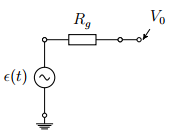
\includegraphics[scale=0.7]{Circuito1-a.png}
    \caption{Divisor de tensão utilizado para medir a resistência interna do gerador Rg.
    ($V_0 $,V) representam as amplitudes das ondas senoidais medidas no osciloscópio.}
    \label{Circuito1a}
    \end{figure}

O gerador de função foi ligado gerando uma onda senoidal em uma frequência aproximada de 100Hz e uma amplitude \textit{Pico-a-pico} de 1V. Depois, com o uso do osciloscópio (com suas escalas devidamente ajustadas) foi medida a Amplitude \textit{Pico-a-Pico} da onda observada.

Depois, um resistor de $R=50$ $\Omega$ foi ligado ao circuito, e com o uso do osciloscópio novamente, a Amplitude \textit{Pico-a-Pico} da onda observada foi medida. (Para garantir o valor da resistência utilizada, ele foi medido com o auxílio de um multímetro na função de ohmímetro). Com esses valores é possível calcular o valor de $R_g $.

Depois, o circuito da \cref{Circuito1.2a} foi montado. O valor de resistência utilizado foi de $R=150$ $\Omega$  e o gerador de função foi ligado no modo de onda senoidal. 

    %%Adicionar FIGURA 1.2A
    \begin{figure}[!htb]
    \centering
    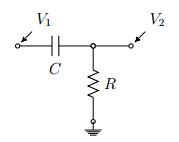
\includegraphics[scale=0.7]{Circuito1-2a.png}
    \caption{Circuito do Filtro Passa Alta.}
    \label{Circuito1.2a}
    \end{figure}

Depois foi utilizado o \textit{MatLAB} com um script fornecido, que fazia a aquisição dos valores de diferença de fase entre a tensão direta na fonte e a tensão no circuito medida no Resistor do Circuito \textit{Passa-alta}.

O mesmo processo foi feito para o Circuito da \cref{Circuito1.2b}, do \textit{Passa-baixa}, e os valores obtidos através do \textit{MatLAB}.

    %%Adicionar FIGURA 1.2B
    \begin{figure}[!htb]
    \centering
    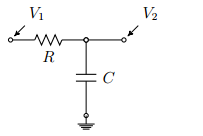
\includegraphics[scale=0.7]{Circuito1-2b.png}
    \caption{Circuito do Filtro Passa Baixa}
    \label{Circuito1.2b}
    \end{figure}

\subsection{Filtros ressonantes}

Na parte B, o circuito da fig. 4 foi estudado de forma a determinar sua frequência de ressonância. O circuito montado inicialmente foi o da \cref{Parte2-1} Para isso, foi utilizado resistores de $R=1 k$$\Omega$ e de $R=150$ $\Omega$.

    %figura 1 a) da parte B (Circuito 4)
    \begin{figure}[!htb]
    \centering
    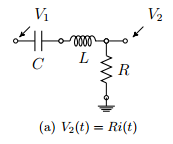
\includegraphics[scale=0.7]{Parte2-1.png}
    \caption{Circuito Ressonante RLC onde $V_2  (t) = R_i (t)$}
    \label{Parte2-1}
    \end{figure}
    
    \begin{figure}[!htb]
    \centering
    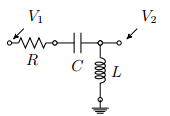
\includegraphics[scale=0.7]{Parte2-2.png}
    \caption{Circuito Ressonante RLC onde $V_2  (t) = L d_i/d_t$}
    \label{Parte2-2}
    \end{figure}

Após a frequência de ressonância ter sido estimada a partir dos valores nominais de capacitância e indutância, o gerador de funções foi ajustado para a frequência de ressonância, e o osciloscópio ajustado para o modo XY (Mostrando as figuras de Lissajous) utilizando-se primeiro o Resistor de $100$ $\Omega$. E depois mantendo-se os mesmos valores na fonte de tensão, trocar o resistor para o de $R=150$ $\Omega$, e depois refinar os valores de tensão aplicados a fim de obter uma reta no gráfico XY do osciloscópio.

Agora, mantendo-se o circuito da \cref{Parte2-1}, e com o auxílio do \textit{MatLAB}, foi feita uma varredura do comportamento do circuito medindo a diferença de fase entre a tensão de entrada, e a tensão que passava pelo circuito.

Depois, os mesmos passos de estimar a frequência, obter as figuras de Lissajous e fazer a varredura com o auxílio do \textit{MatLAB} feitos com a \cref{Parte2-1}, foram feitos com o circuito ressonante da \cref{Parte2-2}.\\

As expressões de $V_1pp$ e $V_2pp$ deduzidas são:\\
$V_1pp (\omega) = e(\omega) * (R + Z_c)/(R_g + R + Z_c)$\\
$V_2pp (\omega) = e(\omega) * Z_C / (R_g + R + Z_c)$

\begin{table}[]
\centering
\caption{Tabela das equações utilizadas}
\label{my-label}
\begin{tabular}{ll}
Rg=R(x1)                          & Equação 1 \\
f0 = 1/(LC)\textasciicircum (1/2) & Equação 2
\end{tabular}
\end{table}

\section{Resultados}
\subsection{Filtro RC passa-alta e passa-baixa}
A partir das varreduras da parte A do experimento, obtemos os gráficos da \cref{Varredura1A}\\
Para a tensão pico-a-pico da fonte: $V_opp &= (1.02 \pm 0.01)V$\\
Tensão pico-a-pico para determinar R_g: V_pp &= (508 \pm 1)mV\\
Resistência interna da fonte: R &= (50.1 \pm 0.1)\Omega\\

\newpage
    \begin{figure}[!htb]
    \centering
    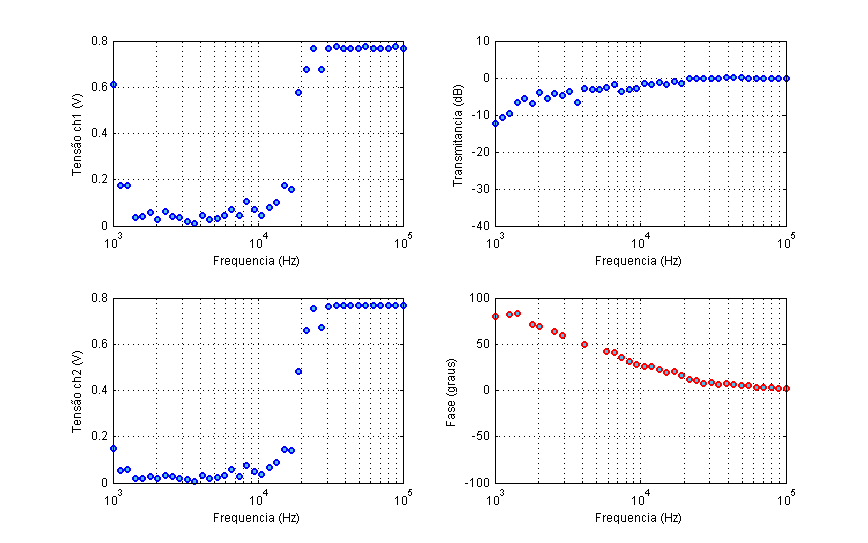
\includegraphics[scale=0.8]{Varredura1A.png}
    \caption{Graficos gerados da Varredura realizada através do \textit{MatLAB} de tensão (Volts), transmitância e diferença de fase, em função da frequência (Hz) da fonte de entrada para o circuito da \cref{Circuito1.2a} da parte 1 do experimento. Filtro Pass-alta}
    \label{Varredura1A}
    \end{figure}

Agora, a partir dos dados obtidos da varredura para o circuito \cref{Circuito1.2b}, obtemos o comportamento observado nos gráficos da \cref{Varredura2B}\\
\newpage
%FIGURA
    \begin{figure}[!htb]
    \centering
    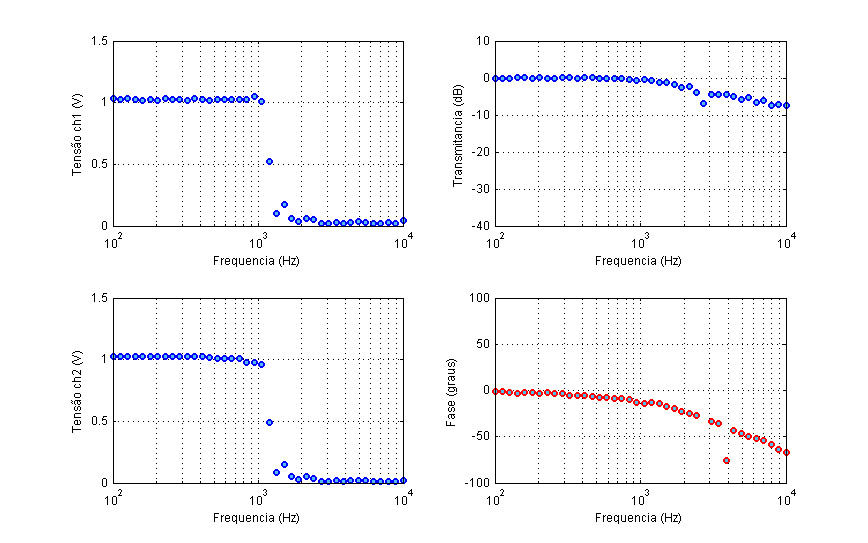
\includegraphics[scale=0.8]{Varredura2B.png}
    \caption{Graficos gerados da Varredura realizada através do \textit{MatLAB} de tensão (Volts), transmitância e diferença de fase, em função da frequência (Hz) da fonte de entrada para o circuito da \cref{Circuito1.2b} da parte 1 do experimento. Filtro Passa-baixa}
    \label{Varredura2B}
    \end{figure}

\subsection{Filtros Ressonantes}

Através da varredura feita com o auxílio do \textit{MatLAB}, para o circuito \cref{}, podemos montar os gráficos da \cref{}

%FIGURA
    \begin{figure}[!htb]
    \centering
    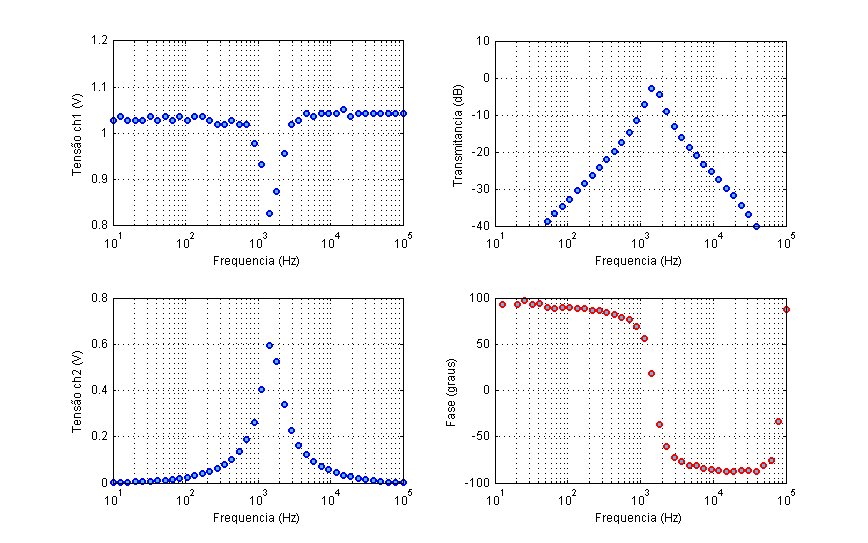
\includegraphics[scale=0.8]{Varredura2AParte2.png}
    \caption{Graficos gerados da Varredura realizada através do \textit{MatLAB} de tensão (Volts), tranmitância(dB) e diferença de fase em função da frequência (Hz). Filtro passa-banda.}
    \label{Varredura2AParte2}
    \end{figure}
    
E com os dados obtidos através da varredura do circuito \cref{} na parte b do experimento, podemos omntar os gráficos de comportamento da \cref{}.

%FIGURA
    \begin{figure}[!htb]
    \centering
    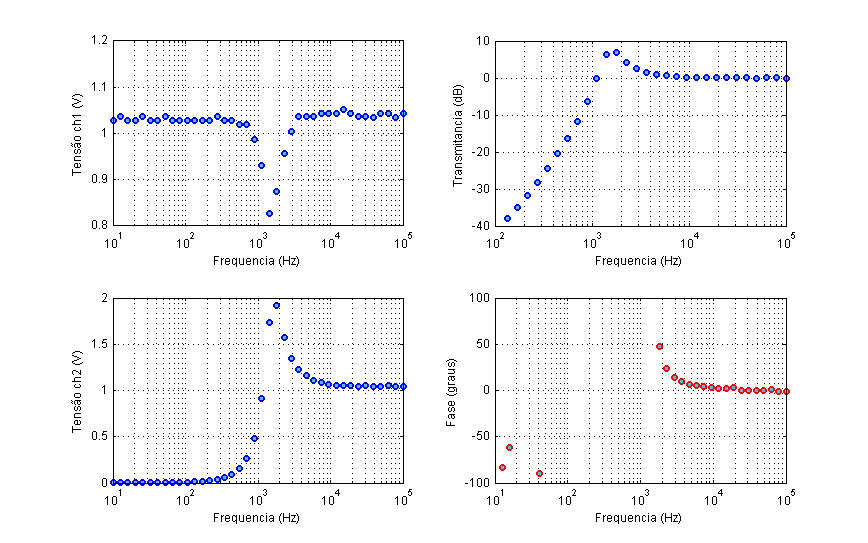
\includegraphics[scale=0.8]{Varredura2BParte2.png}
    \caption{Graficos gerados da Varredura realizada através do \textit{MatLAB} de tensão (Volts), tranmitância(dB) e diferença de fase em função da frequência (Hz)}
    \label{Varredura2BParte2}
    \end{figure}




\section{Análise de Dados}

Com base nos resultados obtidos e aplicando a equação 1, pudemos calcular $R_g \pm \Delta R_g$:\\
$V_opp * R / (R + R_g) = V_pp => R_g = (V_opp * R - V_pp * R)/V_pp = (V_opp - V_pp)*R/V_pp$\\
$\Delta R_g^2 = (R/V_pp)^2 * \Delta V_opp^2 + ((-R*V_pp - (V_opp - V_pp)) * R/V_pp^2)^2 * \Delta V_pp^2 + ((V_opp - V_pp)/V_pp)^2 * \Delta R^2$\\
$=> (R_g \pm \Delta R_g) = (50 \pm 1) \Omega$

%%ITEM C
A partir das informações e dados coletados, podemos gerar um gráfico de $T_d_b$ e $\delta$$_\psi$
\newpage
%FIGURA
    \begin{figure}[!htb]
    \centering
    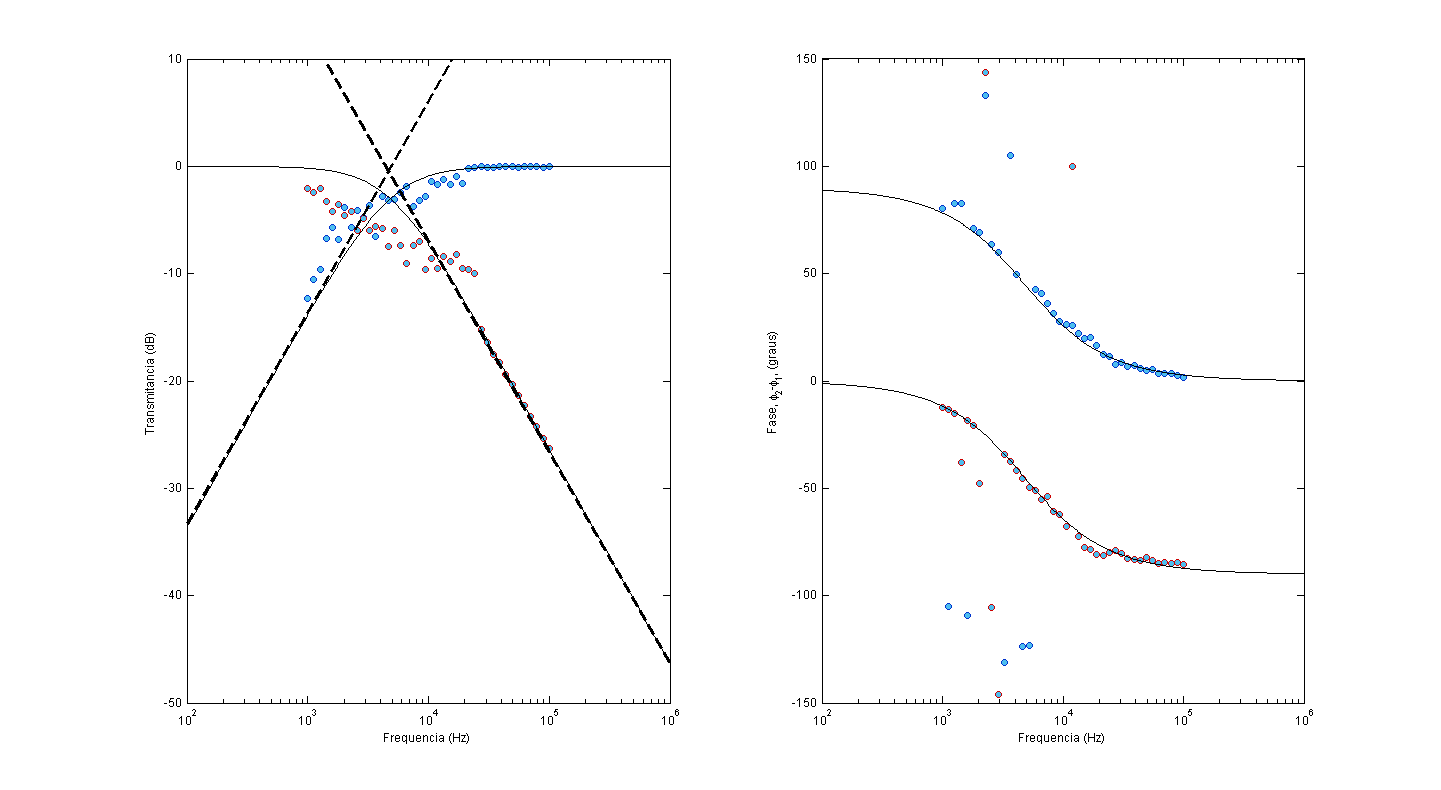
\includegraphics[scale=0.5]{3.png}
    \caption{Diagrama de Bode para a parte 1 do experimento}
    \label{3}
    \end{figure}
    
Através das assíntotas medidas do gráfico, é possível estimas a frequencia de corte para os circuitos. 

Para o circuito passa-baixa está aproximadamente em 1250Hz e para o passa-alta, 11800Hz.

Aparentemente, não tem nada muito discrepante em relaçao à literatura conhecida e o experimento realizado para essa parte.

Com o circuito ressonante RLC, a partir das figuras de Lissajous observadas no osciloscópio, foi possível encontrar um valor mais real para a indutância do capacitor utilizado. O valor nominal da indutância era de (47.91$\pm$0.01)mH e a partir dos dados do experimento foi possível encontrar um valor de (49.34$\pm$0.07)mH.


\section{Discussão}
\subsection{Filtros RC passa-alta e passa-baixa}

Os filtros feitos com circuitos RC podem ter comportmentos distintos. Dentre os circuitos estudados tem-se o comportamento de passa-alta e passa-baixa.

O experimento permitiu compreender que o circuito passa alta, até um limiar chamado de frequencia de corte, não permite a passagem de corrente, e após esse limiar ele passa e transmite o sinal integralmente como seu não houvesse filtro.

Já o circuito passa baixa tem um comportamento contrário e análogo ao passa alta. Ele conduz até um limiar e depois disso ele deixa de transmitir o sinal.

Podemos assiciar os dois circuitos, passa-alte e passa-baixa, de modo que ou ele bloquei uma banda (intervalo) de frequencia, ou que ele permita a transmissao do sinal em uma banda específica. Embora esses circuitos sejam simples eles são de grande aplicabilidade em tratamento de radiofrequencias, sinais e na industrias em geral.

\subsection{Filtros Ressonantes}
O circuito Passa banda, funciona basicamente com a junção de um circuito passa-alte e passa-baixa, baseado em um circuito RLC.

Esse tipo de circuito tem uma frequencia de ressonancia, onde a resposta do capacitor anula a impedancia do indutor, assim a impedancia do circuito passa a ser puramente resistiva, anulando quaisquer diferencas de fase com a fonte.

Ao compararmos os valores das frequências de ressonância $f_0$ medidas usando os resistores de 1k$\Omega$ e 150$\Omega$, pode-se notar que eram de divergentes. Isso se deve ao fato de que, ao utilizarmos um resistor de resistência maior, as variações de tensão provocam variações de corrente relativamente pequenas, mais difíceis de seres medidas. Logo, a medida do resistor maior é mais grosseira, tendo maior erro.
\\
\section{êsão}

Através do experimento realizado, foi possível averiguar o comportamento dos circuitos RC passa-alta e passa-baixa. A resistência interna do gerador de função foi encontrada como sendo  de (50\pm1) $\Omega$, dentro do  valor marcado no equipamento de 50 $\Omega$. Depois no caso dos circuitos RLC ressonantes, também foi possível compreender o fenômeno da passagem de banda e da frequência de ressonância. A frequência de ressonância é próxima da faixa de 1550Hz, para ambos os circuitos RLC montados. 

\section{Instrumentos utilizados}
Os instrumentos utilizados neste experimento foram,
\begin{itemize}
	\item Osciloscópio Tektronix 10002B
	\item Gerador de funções arbitrárias BK Instruments 4052
	\item Multímetro HYX Digital
\end{itemize}

\section{Propagação de erros \label{ap:erros}}
\subsection{Medidas de tensão}
As medidas de tensão foram realizadas utilizando os recursos de medidas automáticas do osciloscópio. Os erros associados às medidas de tensão pico-a-pico do osciloscópio, são pequenos. Segundo o manual do instrumento, a imprecisão da medida de diferença de tensão deve ser calculada como 
\begin{equation}
\Delta V_{pp}=\pm 3\%\text{do valor de leitura + 5\% da escala vertical (V/div)} .
\end{equation}
Nos pontos de menor transmitância mostrados na \cref{fig:exemplo} ($T_{dB}$\approx-40 $ dB$), a menor tensão medida foi $V_{2pp}\approx 10$ mV. Em uma escala de 2 mV/div, o erro da medida seria $\Delta V_{2pp}\approx 0.4$ mV.

\subsection{Resistência interna do gerador}
O erro da resistência interna do gerador foi calculado com base na expressão $R_g=R($V_{1pp}/V_{0pp}-1$)$, sendo $V_{1pp},V_{0pp}$ as tensões pico-a-pico medidas pelo osciloscãpio com o circuito aberto e com um resistor com resistência $R=(148 \pm 5)$ $\Omega$. Portanto o erro associado à resistência interna é dado por,
\begin{equation}
\Delta R_g/R_g= \sqrt{ (\Delta R/R)^2+(\Delta V_{1pp}/V_{1pp})^2+(\Delta V_{0pp}/V_{0pp})^2 }.
\label{eq:erroRg}
\end{equation}
O erro do resistência $\Delta R$ foi calculada seguindo o manual do instrumento, $\pm 1$\% do valor de leitura + 1 dígito. Os erros associados é medidas de tensão pico-a-pico do osciloscópio, apresentadas na \cref{fig:exemplo}, são desprezíveis. Segundo o manual do instrumento a imprecisão da medida de diferença de tensão deve ser calculada como  $\pm3$\% do valor de leitura + 5\% da escala vertical (V/div).  Portanto, mesmo nos pontos com transmitância mais baixa ($T_{dB}\approx-40 $ dB), a menor tensão medida foi $V_{2pp}\approx \max(V_{2pp})/100 = 10$ mV. Em uma escala de 2 mV/div, o erro da medida seria $\Delta V_{2pp}\approx 0.4$ mV.


%*********************************************
%REFERENCIAS BIBLIOGRAFICAS
%*********************************************
\begin{thebibliography}{10}

\bibitem{apostila}Gustavo Wiederhecker e colaboradores, \textsl{Roteiros de F429 - Corrente alternada e óptica.} Compilado em 29 de agosto de 2016.

\bibitem{tabelastex}\url{http://www.tablesgenerator.com}

\end{thebibliography}

%*********************************************
%FIM DO DOCUMENTO
%******************
\end{document}